\documentclass[../main.tex]{subfiles}
\begin{document}
\section{Results}\label{results}
%oppgave 5b)
\subsection{Euler and Verlet without oo}
In order to make sure that our algorithm is running correctly, we will start solving the differential equation using both Euler's and Verlet's method without using object oriented(oo) code. The algorithms used to calculate the two are located in the following folders (\href{https://github.com/kmaasrud/Project-5/tree/master/code/Earth-Sun_Euler-FWD}{(Euler)} and \href{https://github.com/kmaasrud/Project-5/tree/master/code/Earth-Sun_Verlet}{(Verlet)}

\begin{figure}[!h]
  \centering
  \parbox{5cm}{
  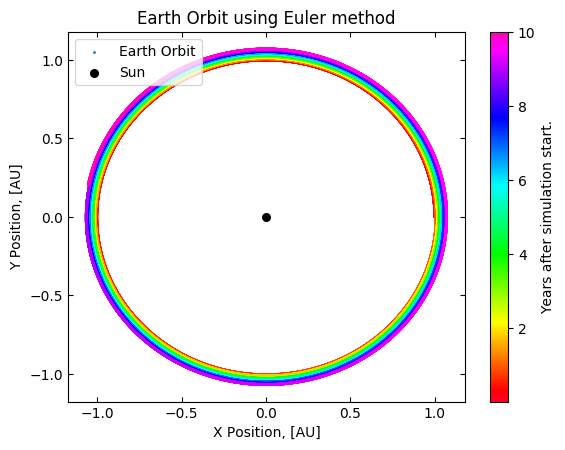
\includegraphics[width=5cm]{EarthOrbit_Euler.png}
  \caption{Earth orbit around the Sun using Eulers method}
  \label{fig:EarthOrbit_Euler}}
  \qquad
  \begin{minipage}{5cm}
    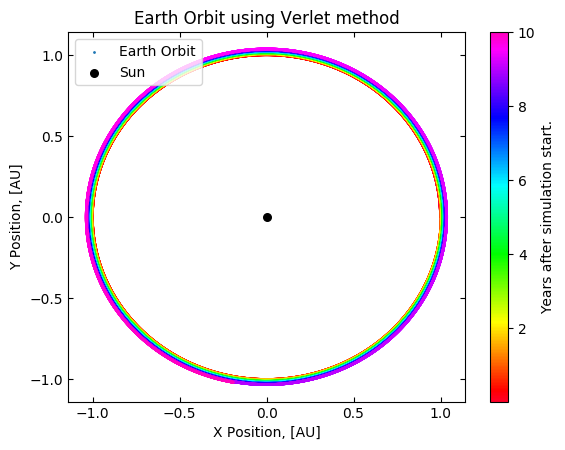
\includegraphics[width=5cm]{EarthOrbit_Verlet.png}
    \caption{Earth orbit around the Sun using Verlet's method}
    \label{fig:EarthOrbit_Verlet}
  \end{minipage}
  \end{figure}
\FloatBarrier

%skriv litt om programflow

%oppgave 5c)
The stability is tested using different timesteps
\begin{figure}[!h]
  \centering
  \parbox{5cm}{
  \includegraphics[width=5cm]{}
  \caption{Timestep: }
  \label{fig:}}
  \qquad
  \begin{minipage}{5cm}
    \includegraphics[width=5cm]{}
    \caption{Timestep: }
    \label{fig:}
  \end{minipage}
  \end{figure}
\FloatBarrier

Initial value for velocity giving circular orbits.
Stability as function of different timesteps- plots of earths position.

Concercation of energy- kinetic + potential

%oppgave 5f)
Sammenlign resultetene med de tidligere.


\end{document}
